\documentclass[12pt]{beamer}
\usepackage{amsmath}
\usepackage[utf8]{inputenc}
\usepackage{apacite}

\usetheme{Singapore}
\usepackage[style=british]{csquotes}

\def\signed #1{{\leavevmode\unskip\nobreak\hfil\penalty50\hskip1em
		\hbox{}\nobreak\hfill #1%
		\parfillskip=0pt \finalhyphendemerits=0 \endgraf}}

\newsavebox\mybox
\newenvironment{aquote}[1]
{\savebox\mybox{#1}\begin{quote}\openautoquote\hspace*{-.7ex}}
	{\unskip\closeautoquote\vspace*{1mm}\signed{\usebox\mybox}\end{quote}}


\DeclareMathOperator*{\argmin}{arg\,min}
\usepackage{soul}


	\title{Factor Strength and Factor Selection }
	\subtitle{An Application to U.S. Stock Market}

		\date{\today}
		\author[author]{Zhiyuan Jiang\\
			28710967\\
			[10mm]
            Supervisors: Dr Natalia Bailey \\ 
			\hspace{18.5mm} 
			Dr David Frazier}
		
		
\begin{document}
	
\frame[plain]{\titlepage}

%-------------------------------------------------------------------------------------------------------------------------------------------------------------------------------%
%-------------------------------------------------------------------------------------------------------------------------------------------------------------------------------%
\section{Introduction and Motivation}

\begin{frame}{Motivation}
	
Capital Asset Pricing Model (CAPM) is the benchmark of risk pricing.
\[r_{it} - r_{ft} = a_i + \beta_{im}(r_{mt} - r_{ft}) + \sum_{j=1}^{k}\beta_{ij}f_{jt} + \varepsilon_{it} \]

\begin{columns}
	\begin{column}{0.5\textwidth}
\begin{itemize}
\item $r_{it}$: asset's return
\item $r_{ft}$: risk free return
\item $a_i$: constant/intercept
\item $\beta_{im}$: market factor loading
\end{itemize}
	\end{column}
	\begin{column}{0.5\textwidth}  
		\begin{center}
\begin{itemize}
\item $r_{mt}$: market return 
\item$\beta_{ij}$: risk factor loading
\item $f_{jt}$: risk factor
\item $\varepsilon_{it}$: stochastic error
\end{itemize}
		\end{center}
	\end{column}
\end{columns}
\begin{itemize}
\item{\bf Add factors to enhance risk pricing.}
\item{\bf  New factors are booming }
\end{itemize}

\end{frame}




\begin{frame}[plain]
	\begin{figure}
\includegraphics[scale = 0.5]{figure/factor_growth.png}
\caption{Factor amount growing through the year. }
	\cite{Harvey2019}\\
	\end{figure}
\end{frame}

\begin{frame}
\begin{aquote}{\citeNP{Cochrane2011}}
	We have a lot of questions to answer: \\
	Firstly, which characteristics really provide \textbf{independent} information about average returns? Which are subsumed by others ?
\end{aquote}

\begin{figure}
	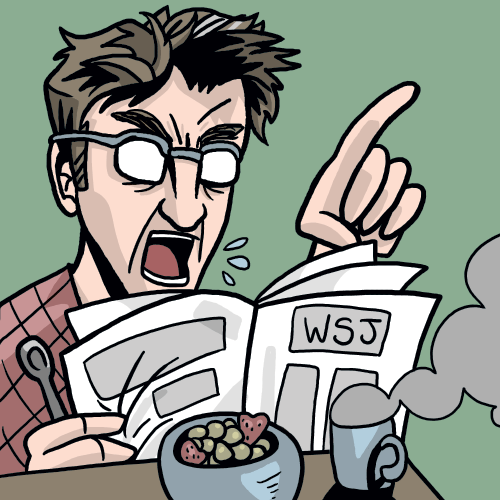
\includegraphics[scale = 0.2]{figure/cochrane.png}
\end{figure}
\end{frame}



\begin{frame}
	\frametitle{Factor Strength}
	The research interest is pricing risk, so factor strength matter.

	Consistency of risk pricing is dependent on the strength of factor \cite{Pesaran2019}
	


	Strong factor $\Rightarrow$ price more asset's risk $\Rightarrow$ generate more significantly loadings.
	
		Factor strength is defined in terms of factor loading \cite{Bailey2020} as follow.

	 Assume we have N different assets.
%	If a factor $x_j$ has strength $\alpha_j$, we let this factor regress with N different assets.
	\begin{align*}
	|\beta_j| &> CV , j = 1, 2, 3, \cdots, [N^{\alpha_j}]\\
	|\beta_j |&= 0, j = [N^{\alpha_j} ]+1 ,[N^{\alpha_j}]  +2, [N^{\alpha_j}] +3, \cdots, N
	\end{align*}
\end{frame}
\begin{frame}
\frametitle{Introduction and Motivation}
But some problems exist among all those factors.\\


\begin{itemize}
\item Including Factor without correlation with return in FM first-regression\cite{Fama1973} will yield misleading second regression result \cite{Kan1999}
\item If the factor loading is small, estimated risk premia will be spurious \citeA{Kleibergen2009}
\end{itemize}

Reference to this problem is made in the literature:

\citeA{Kan1999}, \citeA{Kleibergen2009}, \citeA{Kleibergen2015}, \citeA{Gospodinov2017}, \citeA{Anatolyev2018}

\end{frame}


%-------------------------------------------------------------------------------------------------------------------------------------------------------------------------------%
%-------------------------------------------------------------------------------------------------------------------------------------------------------------------------------%
	\section{Related Literature}
	\begin{frame}
\frametitle{Literature}
\begin{itemize}
	%\item{\bf Consequences of including weak factors}\\
	%\citeA{Kan1999}, \citeA{Kleibergen2009}, \citeA{Kleibergen2015}, \citeA{Gospodinov2017}, \citeA{Anatolyev2018}
	\item {\bf Identify factors}\\
	\citeA{Harvey2015}, \citeA{McLean2016}, \citeA{Harvey2017}, \citeA{Barillas2018},\citeA{Pukthuanthong2019}
	\item {\bf Using machine learning method}\\
	\citeA{Rapach2013}, \citeA{Feng2019},\citeA{Gu2020}, \citeA{Lettau2020}, \citeA{Freyberger2020}, \citeA{Kozak2020}
	\end{itemize}
	\end{frame}
	
	
	
	
	
%	\begin{frame}
%\frametitle{Identify Useful Factors}
%There are a bunch of literatures and researches aiming identify useful factors.
%\begin{enumerate}
%\item \citeA{Harvey2015} exams over 300 factors, and suggest to arise the p-value threshold to 3 to eliminate some new factors turns to be significant purely by luck.
%\item \citeA{Harvey2017} introduce a bootstrap method 
%\item \citeA{Barillas2018} use Bayes procedure to find useful factor
%\item \citeA{Pukthuanthong2019} defined a protocol to identify priced factor.
%\end{enumerate}
	%\end{frame}

%\begin{frame}
%	\frametitle{Identify Useful Factor}
%A recent studies shows that using Machine Learning methods in asset pricing can bring huge benefits \cite{Gu2020}\\
%\begin{itemize}
%\item Better predict accuracy
%\item Improved efficiency
%\end{itemize}
%\end{frame}

%\begin{frame}
%	\frametitle{Identify Useful Factor}
%Some researchers already started using Machine Learning algorithms, especially Lasso, a factor selection algorithm.
%\begin{enumerate}
%\item \citeA{Rapach2013} using Lasso to find factor for predicting global stock market return.
%\item \citeA{Feng2019} used a improved double-selected method in factor selection
%\item Because Lasso has some limitation, \citeA{Huang2010} implied a group lasso method, trying to overcome such shortcoming.
%\end{enumerate}
%\end{frame}

%-------------------------------------------------------------------------------------------------------------------------------------------------------------------------------%
%-------------------------------------------------------------------------------------------------------------------------------------------------------------------------------%


	\section{Methodology}

\begin{frame}
\frametitle{Main Problem}
This project faces two challenges:
\begin{enumerate}
\item	 High dimensions of data group\\
How to identify the significant one. $\Rightarrow$ \alert{use factor strength as criteria.}
\item 	Correlation among factors \\
Traditional variable selection algorithm (Lasso) can not handle this.$\Rightarrow$ Will use \alert{elastic net} techniques
\end{enumerate}
\end{frame}

%\begin{frame}
%\frametitle{Methodology}
%For each of the problems mentioned above
%\begin{enumerate}
%\item Calculate the factor strength, only focus on factor with certain strength
%\item Use Elastic Net model, overcome the correlation problem 
%\end{enumerate}
%\end{frame}
	
\begin{frame}
\frametitle{Elastic Net}
Introduce by \citeA{Zou2005}, is a improved method to select factor.

Considering the following loss function:

	\[   \hat{\beta}_{ij}  = \argmin_{\beta_{ij}}\{\sum_{i = 1}^{n}[(r_{it} - r_{ft}) - \beta_{ij }f_{jt}]^2 + \lambda_2\sum_{i = 1}^{n}\beta_{ij}^2  + \lambda_1\sum_{i = 1}^{n}|\beta_{ij}|     \}    \]
	
	The $L_1$ norm $\sum_{i = 1}^{n}|\beta_{ij}|$ helps select the factor, reduce redundancy.\\
    The $L_2$ norm $\sum_{i = 1}^{n}\beta_{ij}^2 $ helps handle the correlation.

\end{frame}


%-------------------------------------------------------------------------------------------------------------------------------------------------------------------------------%
%-------------------------------------------------------------------------------------------------------------------------------------------------------------------------------%


\section{Data and Methods}


\begin{frame}
	\frametitle{Preliminary Result}
Use Monte Carlo simulation to study the property of estimated factor strength.\\
\[ \hat{\alpha} = \begin{cases}
1+\frac{\ln(\hat{\pi}_{nT})}{\ln n} & \text{if}\; \hat{\pi}_{nT} > 0,\\
0, & \text{if}\; \hat{\pi}_{nT} = 0.
\end{cases} \]
\begin{itemize}
\item Overestimates occurs when strength is low $\alpha = 0.5, \hat{\alpha} \approx 0.7$
\item But the precision improved with strength increase $\alpha = 0.7, \hat{\alpha} = 0.8$
\item When we have the strong factor, we have the unbiased estimator $\alpha = \hat{\alpha} = 1$
\end{itemize}
	
\end{frame}

\begin{frame}
\frametitle{Data}
The data set contains two part:
\begin{itemize}
\item {\bf Assets}: Stocks from Standard \& Poor (S\&P) 500 index companies\\
\subitem Three year U.S. t-bill
\subitem Average return of U.S. stock market
\item {\bf Factor}: 145 risk factors plus one market factor.\\
\end{itemize}

Thirty year time period: Jan 1987 - Dec 2007.\\
Data set into three subsamples: 10/20/30 years.\\
\end{frame}

%-------------------------------------------------------------------------------------------------------------------------------------------------------------------------------%
%-------------------------------------------------------------------------------------------------------------------------------------------------------------------------------%
\begin{frame}
	\centering	
\huge{ Thanks for listening\\}
\end{frame}


%-------------------------------------------------------------------------------------------------------------------------------------------------------------------------------%
%-------------------------------------------------------------------------------------------------------------------------------------------------------------------------------%
\begin{frame}[allowframebreaks]
	\frametitle{Bibliography}
	\bibliographystyle{apacite}
{\footnotesize\bibliography{library.bib}}
\end{frame}
\end{document}